\documentclass[16pt]{beamer}
\usepackage[utf8]{inputenc}
\usepackage[T1]{fontenc}
\usepackage{graphicx}
\usepackage[polish]{babel}
\usepackage{url}
\usepackage{fancyvrb}
\usepackage{color}

\newcommand\at{@}
\newcommand\lb{[}
\newcommand\rb{]}
\newcommand\PYbg[1]{\textcolor[rgb]{0.00,0.50,0.00}{\textbf{#1}}}
\newcommand\PYbf[1]{\textcolor[rgb]{0.73,0.40,0.53}{\textbf{#1}}}
\newcommand\PYbe[1]{\textcolor[rgb]{0.40,0.40,0.40}{#1}}
\newcommand\PYbd[1]{\textcolor[rgb]{0.73,0.13,0.13}{#1}}
\newcommand\PYbc[1]{\textcolor[rgb]{0.00,0.50,0.00}{\textbf{#1}}}
\newcommand\PYbb[1]{\textcolor[rgb]{0.40,0.40,0.40}{#1}}
\newcommand\PYba[1]{\textcolor[rgb]{0.00,0.00,0.50}{\textbf{#1}}}
\newcommand\PYaJ[1]{\textcolor[rgb]{0.73,0.13,0.13}{#1}}
\newcommand\PYaK[1]{\textcolor[rgb]{0.00,0.00,1.00}{#1}}
\newcommand\PYaH[1]{\fcolorbox[rgb]{1.00,0.00,0.00}{1,1,1}{#1}}
\newcommand\PYaI[1]{\textcolor[rgb]{0.69,0.00,0.25}{#1}}
\newcommand\PYaN[1]{\textcolor[rgb]{0.00,0.00,1.00}{\textbf{#1}}}
\newcommand\PYaO[1]{\textcolor[rgb]{0.00,0.00,0.50}{\textbf{#1}}}
\newcommand\PYaL[1]{\textcolor[rgb]{0.73,0.73,0.73}{#1}}
\newcommand\PYaM[1]{\textcolor[rgb]{0.74,0.48,0.00}{#1}}
\newcommand\PYaB[1]{\textcolor[rgb]{0.00,0.25,0.82}{#1}}
\newcommand\PYaC[1]{\textcolor[rgb]{0.67,0.13,1.00}{#1}}
\newcommand\PYaA[1]{\textcolor[rgb]{0.00,0.50,0.00}{#1}}
\newcommand\PYaF[1]{\textcolor[rgb]{1.00,0.00,0.00}{#1}}
\newcommand\PYaG[1]{\textcolor[rgb]{0.10,0.09,0.49}{#1}}
\newcommand\PYaD[1]{\textcolor[rgb]{0.25,0.50,0.50}{\textit{#1}}}
\newcommand\PYaE[1]{\textcolor[rgb]{0.63,0.00,0.00}{#1}}
\newcommand\PYaZ[1]{\textcolor[rgb]{0.00,0.50,0.00}{\textbf{#1}}}
\newcommand\PYaX[1]{\textcolor[rgb]{0.00,0.50,0.00}{#1}}
\newcommand\PYaY[1]{\textcolor[rgb]{0.73,0.13,0.13}{#1}}
\newcommand\PYaR[1]{\textcolor[rgb]{0.10,0.09,0.49}{#1}}
\newcommand\PYaS[1]{\textcolor[rgb]{0.25,0.50,0.50}{\textit{#1}}}
\newcommand\PYaP[1]{\textcolor[rgb]{0.49,0.56,0.16}{#1}}
\newcommand\PYaQ[1]{\textcolor[rgb]{0.40,0.40,0.40}{#1}}
\newcommand\PYaV[1]{\textcolor[rgb]{0.00,0.00,1.00}{\textbf{#1}}}
\newcommand\PYaW[1]{\textcolor[rgb]{0.73,0.13,0.13}{#1}}
\newcommand\PYaT[1]{\textcolor[rgb]{0.50,0.00,0.50}{\textbf{#1}}}
\newcommand\PYaU[1]{\textcolor[rgb]{0.82,0.25,0.23}{\textbf{#1}}}
\newcommand\PYaj[1]{\textcolor[rgb]{0.00,0.50,0.00}{#1}}
\newcommand\PYak[1]{\textcolor[rgb]{0.73,0.40,0.53}{#1}}
\newcommand\PYah[1]{\textcolor[rgb]{0.63,0.63,0.00}{#1}}
\newcommand\PYai[1]{\textcolor[rgb]{0.10,0.09,0.49}{#1}}
\newcommand\PYan[1]{\textcolor[rgb]{0.67,0.13,1.00}{\textbf{#1}}}
\newcommand\PYao[1]{\textcolor[rgb]{0.73,0.40,0.13}{\textbf{#1}}}
\newcommand\PYal[1]{\textcolor[rgb]{0.25,0.50,0.50}{\textit{#1}}}
\newcommand\PYam[1]{\textbf{#1}}
\newcommand\PYab[1]{\textit{#1}}
\newcommand\PYac[1]{\textcolor[rgb]{0.73,0.13,0.13}{#1}}
\newcommand\PYaa[1]{\textcolor[rgb]{0.50,0.50,0.50}{#1}}
\newcommand\PYaf[1]{\textcolor[rgb]{0.25,0.50,0.50}{\textit{#1}}}
\newcommand\PYag[1]{\textcolor[rgb]{0.40,0.40,0.40}{#1}}
\newcommand\PYad[1]{\textcolor[rgb]{0.73,0.13,0.13}{#1}}
\newcommand\PYae[1]{\textcolor[rgb]{0.40,0.40,0.40}{#1}}
\newcommand\PYaz[1]{\textcolor[rgb]{0.00,0.63,0.00}{#1}}
\newcommand\PYax[1]{\textcolor[rgb]{0.60,0.60,0.60}{\textbf{#1}}}
\newcommand\PYay[1]{\textcolor[rgb]{0.00,0.50,0.00}{\textbf{#1}}}
\newcommand\PYar[1]{\textcolor[rgb]{0.10,0.09,0.49}{#1}}
\newcommand\PYas[1]{\textcolor[rgb]{0.73,0.13,0.13}{\textit{#1}}}
\newcommand\PYap[1]{\textcolor[rgb]{0.00,0.50,0.00}{#1}}
\newcommand\PYaq[1]{\textcolor[rgb]{0.53,0.00,0.00}{#1}}
\newcommand\PYav[1]{\textcolor[rgb]{0.00,0.50,0.00}{\textbf{#1}}}
\newcommand\PYaw[1]{\textcolor[rgb]{0.40,0.40,0.40}{#1}}
\newcommand\PYat[1]{\textcolor[rgb]{0.10,0.09,0.49}{#1}}
\newcommand\PYau[1]{\textcolor[rgb]{0.40,0.40,0.40}{#1}}


\usetheme{Pittsburgh}
\usenavigationsymbolstemplate{} % turn off navigation icons
\setbeamercovered{transparent}

\author{Silesian Ruby Users Group\\
  \footnotesize{Jakub Kuźma}}
\title{RIA development using YUI 3 and Rails 3}

\begin{document}

\frame{\titlepage}

\begin{frame}
  \frametitle{Introduction}
  \begin{center}
    Rich Internet Application?
  \end{center}
\end{frame}

\begin{frame}
  \frametitle{Contract bridge - auction}
  \begin{figure}
    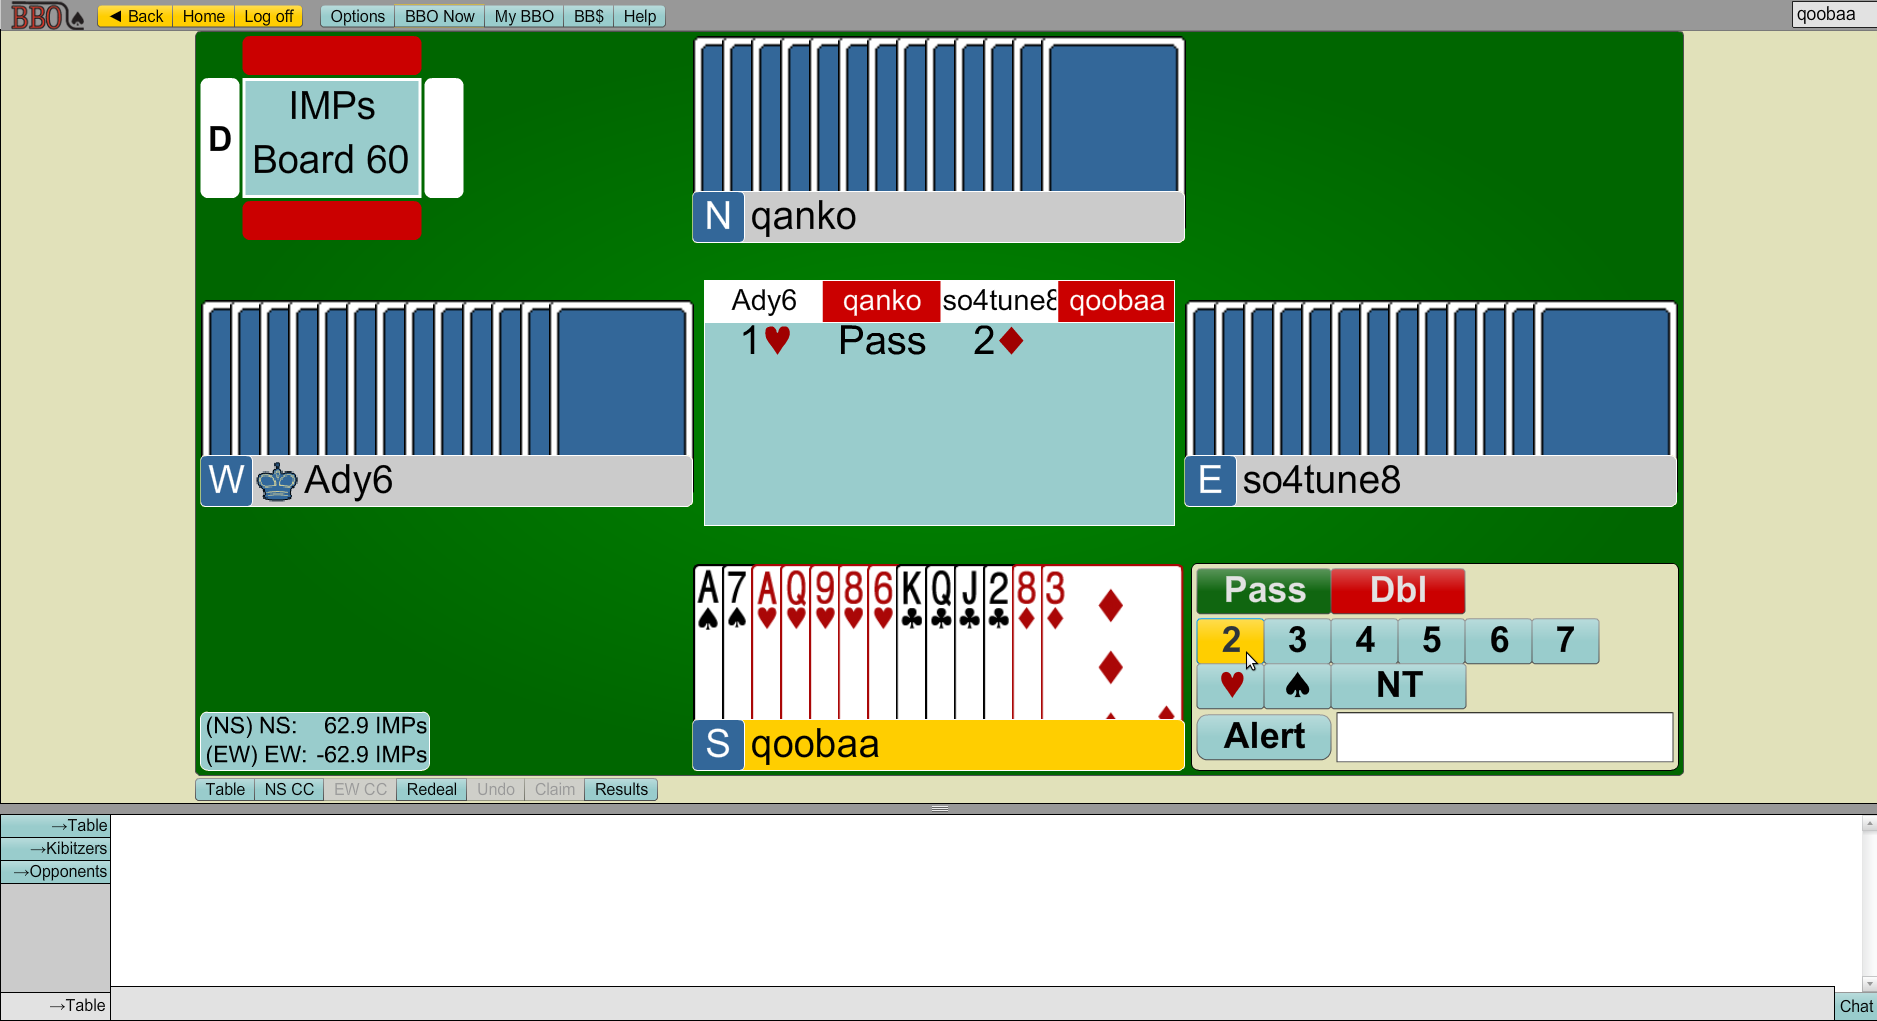
\includegraphics[width=\linewidth]{bbo-auction.png}
  \end{figure}
\end{frame}

\begin{frame}
  \frametitle{Contract bridge - play}
  \begin{figure}
    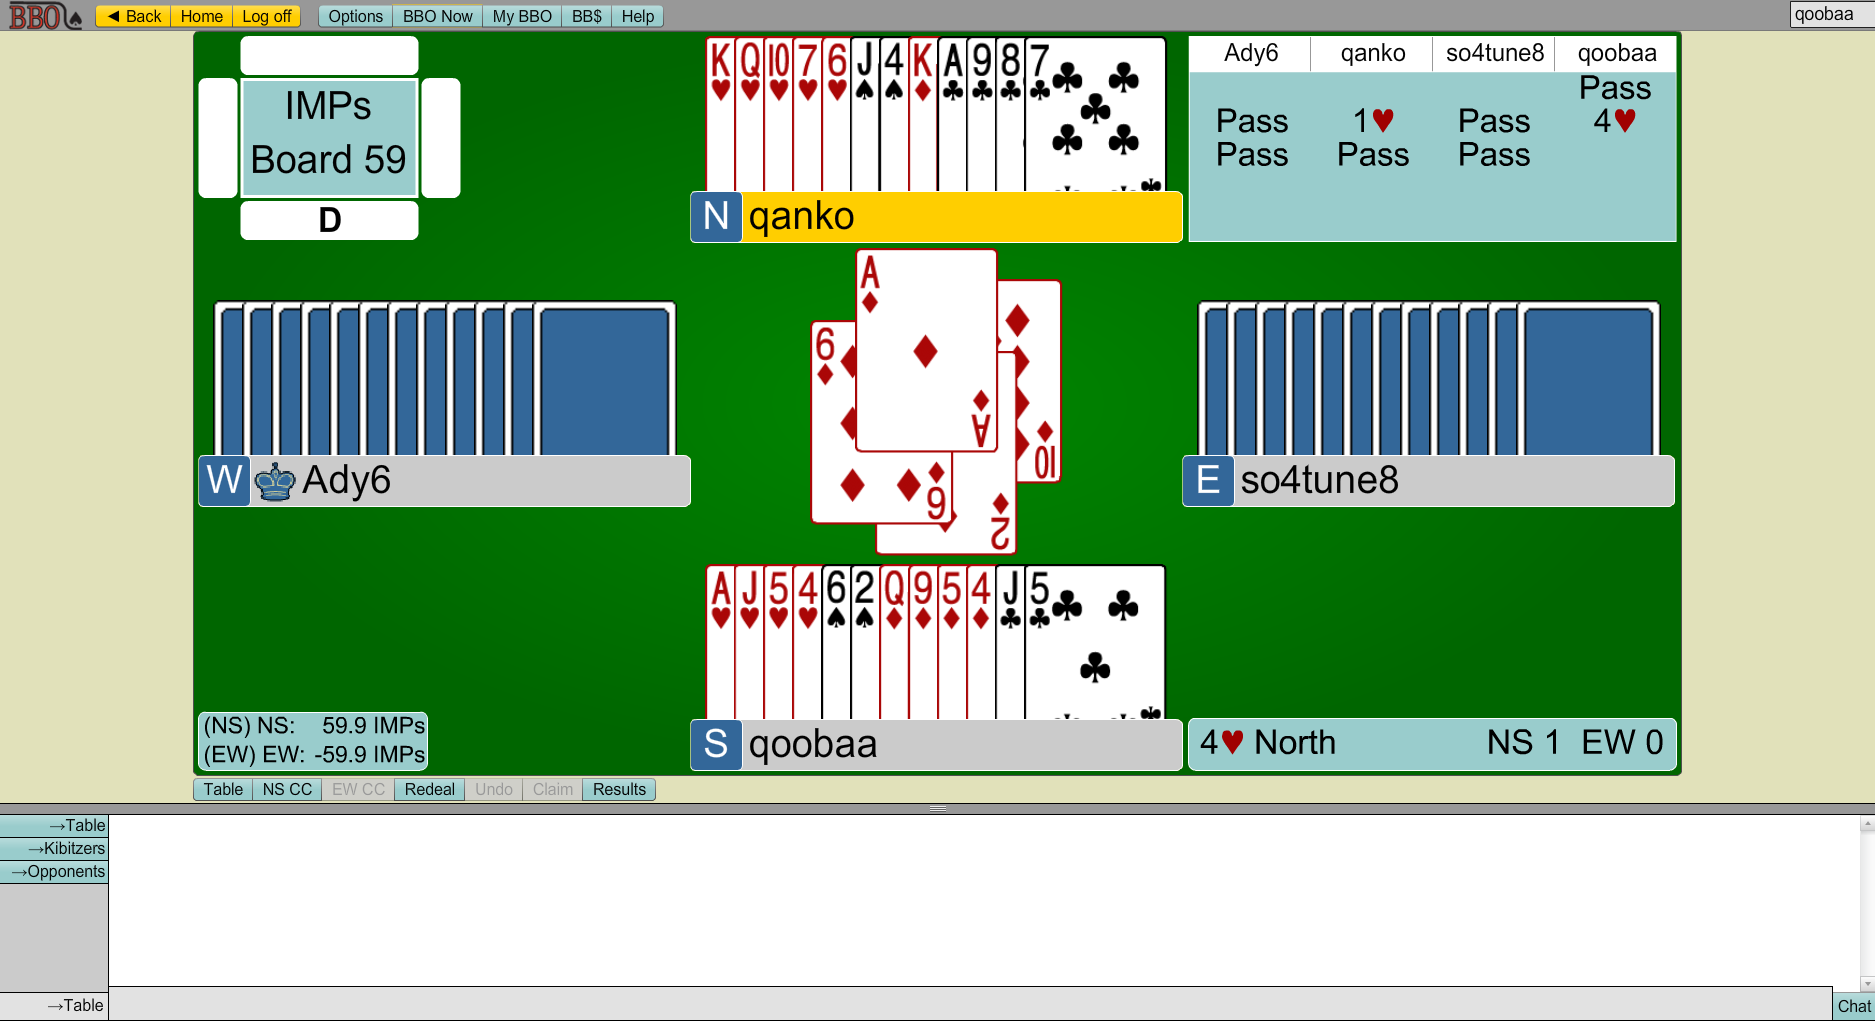
\includegraphics[width=\linewidth]{bbo-play.png}
  \end{figure}
\end{frame}

\begin{frame}
  \frametitle{Requirements}
  \begin{itemize}
  \item client-server communication without refreshing page
  \item client side validation
  \item interface composed of small, independent elements
  \end{itemize}
\end{frame}

\begin{frame}
  \frametitle{jQuery}
  \begin{center}
    ridiculously easy AJAX, event handling, DOM manipulation
  \end{center}
\end{frame}

\begin{frame}
  \frametitle{jQuery UI}
  \begin{center}
    jQuery UI for RIA is like jQuery for AJAX development
  \end{center}
\end{frame}

\begin{frame}
  \frametitle{YUI}
  \begin{figure}
    
\includegraphics[width=0.8\linewidth]{yui.jpg}
  \end{figure}
\end{frame}

\begin{frame}
  \frametitle{YUI 3}
  \begin{itemize}
  \item Developer Tools
  \item Core
  \item Utilities
  \item Component Infrastructure
  \item Widgets
  \item Plugins
  \end{itemize}
\end{frame}

\begin{frame}
  \frametitle{Component Infrastructure}
  \begin{itemize}
  \item Attribute
  \item Base
  \item Widget
  \item Plugin
  \end{itemize}
\end{frame}

\begin{frame}
  \frametitle{Attribute}
  \begin{itemize}
  \item getters, setters, validation
  \item attributeChange event
  \item object cloning
  \item nested objects support (i.e. strings.messages.hello)
  \end{itemize}
\end{frame}

\begin{frame}[fragile]
  \frametitle{Attribute - example}
  \input{attribute}
\end{frame}

\begin{frame}[fragile]
  \frametitle{Attribute - usage}
  \input{attribute-usage}
\end{frame}

\begin{frame}
  \frametitle{Base}
  \begin{itemize}
  \item constructor and destructor
  \item attributes
  \item event target
  \item extension and plugin support
  \end{itemize}
\end{frame}

\begin{frame}[fragile]
  \frametitle{Base - example}
  \input{base}
\end{frame}

\begin{frame}
  \frametitle{Widget}
  \begin{itemize}
  \item HTML Parser
  \item renderUI
  \item bindUI
  \item syncUI
  \item boundingBox, contentBox
  \end{itemize}
\end{frame}

\begin{frame}[fragile]
  \frametitle{Widget - example}
  \begin{footnotesize}
    \input{widget}
  \end{footnotesize}
\end{frame}

\begin{frame}
  \frametitle{Plugin}
  \begin{itemize}
  \item unobtrusively enhance objects (aka hosts)
  \item afterHostEvent, beforeHostMethod, etc.
  \end{itemize}
\end{frame}

\begin{frame}[fragile]
  \frametitle{Plugin - example}
  \begin{footnotesize}
    \input{plugin}
  \end{footnotesize}
\end{frame}

\begin{frame}
  \frametitle{Custom Events}
  \begin{itemize}
  \item DOM independent
  \item same API and behavior (bubbling - stopPropagation, defaultFn - preventDefault)
  \end{itemize}
\end{frame}

\begin{frame}
  \frametitle{Other stuff}
  \begin{itemize}
  \item more array utilities: every, find, reduce, etc.
  \item language helpers: isArray, isValue, isString, etc.
  \item OOP (augment, extend, bind, rbind)
  \item YUI 3 Gallery
  \end{itemize}
\end{frame}

\begin{frame}
  \frametitle{Rails 3}
  \begin{itemize}
  \item ordinary web application (authentication, statistics, etc.)
  \item API (responders rock)
  \item validating user actions
  \end{itemize}
\end{frame}

\begin{frame}
  \frametitle{node.js}
  \begin{itemize}
  \item YUI3 is CommonJS
  \item replace Get module (require instead of <script>)
  \item DOM support by jsdom
  \end{itemize}
\end{frame}

\begin{frame}
  \frametitle{Resources}
  \begin{itemize}
  \item YUI 3\\\url{http://developer.yahoo.com/yui/3/}
  \item Bridge App\\\url{http://bridge.heroku.com/}
  \item Bridge App - source\\\url{http://github.com/morgoth/bridge/}
  \item underscore.js\\\url{http://documentcloud.github.com/underscore/}
  \item mustache.js\\\url{http://github.com/janl/mustache.js/}
  \end{itemize}
\end{frame}

\begin{frame}
  \begin{figure}
    
\includegraphics[width=\linewidth]{drogus.png}
  \end{figure}
\end{frame}

\begin{frame}
  \begin{center}
    \Huge{Questions?}
  \end{center}
\end{frame}

\end{document}
